\chapter{Marco Teórico}

En el presente capítulo se describen conceptos y patrones utilizados para el desarrollo del proyecto de patantía, los cuales fueron seleccionados siguiendo los criterios de usabilidad, mantenibilidad, escalabilidad y portabilidad.

    \section{Modelo Vista Controlador (MVC)}
    
    El Modelo-Vista-Controlador es un patrón de arquitectura de \textit{software} que separa el modelo (Objetos de negocio) la vista (Interfaz con el usuario u otros sistemas) y el controlador (Manejo de la informacion de negocio)\cite{MVC-tiw}.
    
    Específicamente, cada componente tiene una asignación independiente de los demás componentes. Estas son:
    
    \begin{enumerate}
        \item \textbf{Modelo}
            \begin{itemize}
                \item Almacenamiento de los datos.
                \item Estado del sistema.
                \item Recuperación de errores a nivel de datos.
            \end{itemize}
        \item \textbf{Vista}
            \begin{itemize}
                \item Presentación del modelo.
                \item Puede acceder al modelo pero no cambiar su estado.
            \end{itemize}
        \item \textbf{Controlador}
            \begin{itemize}
                \item Reaccionar a las peticiones del cliente.
                \item Comunicar al modelo de las acciones ejecutadas.
                \item Direccionar a las vistas requeridas del lado del cliente.
            \end{itemize}
    \end{enumerate}
    
    \begin{figure}[htbp!]
        \begin{center}
            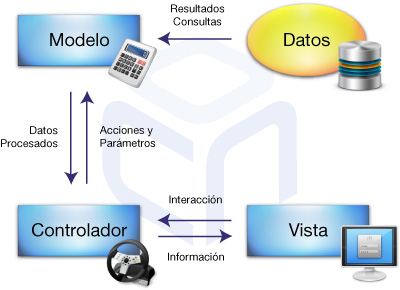
\includegraphics[width=.8\textwidth]{figures/Arquitectura-MVC}
        \end{center}
        \caption{Representación gráfica del patrón Modelo Vista Controlador\cite{MVC-imagen}}
        \label{mvc-image}
    \end{figure}
    
    \section{Arquitectura Orientada a Servicios}
    SOA por sus siglas en inglés, \textit{Service Oriented Architecture}. Es una filosofía de desarrollo la cual actúa como una guía de diseño y facilita el mismo orientado a la escalabilidad del sistema, esto es: facilita las actializaciones de uno o varios de los componentes MVC y minimiza el efecto que dicha actualización tiene sobre los demás.
    
    Según Gartner\cite{SOA-libroGartner} y González Quiroga\cite{SOA-tesis}, la incorporación de SOA empieza en las empresas hacia 2003, por las siguiente razones:
    
    \begin{itemize}
        \item La incesante presión de los negocios para la agilidad. Cuando una empresa quiere
        modificar sus procesos, productos o servicios, no puede permitirse el lujo de esperar por
        mucho tiempo. Debe ser posible cambiar la forma de aplicación de los sistemas de
        trabajo simplemente modificando los componentes que ya están en uso, en lugar de
        comprar o codificar nuevos componentes o sistemas enteros desde cero.
        
        \item La flexibilidad de la arquitectura SOA basada en Servicios Web de apoyo a múltiples
        aplicaciones.
        
        \item  La aceptación unánime de proveedores de los estándares de Servicios Web,
        especialmente de Simple Object Access Protocol (SOAP) y Web Service Description
        Language (WSDL)\cite{SOA-libroGartner}
        
    \end{itemize}
    
    SOA se basa en capas, cada una servicios a la siguiente y sus procedimientos internos se mantienen ocultos a las demás capas. Con esto se generan APIs de acceso estandarizado y son independientes de las tecnologías utilizadas en el desarrollo.
    
    En \textit{Service Oriented Architecture}\cite{SOA-msdn} definen SOA usando el poema de Saxe sobre los ciegos y el elfante.
    
    "Seis ciegos de Indostan se encuentran con un elefante, cada uno describe el elefante de forma diferente porque se ve influenciado por sus propias experiencias (Ver figura \ref{elefante-saxe})
    
    \begin{itemize}
        \item Quien le toca la trompa cree que es una serpiente.
        \item Quien le toca los colmillos cree que son lanzas.
        \item Quien le toca las orejas cree que son abanicos.
        \item Quien le toca la panza cree que es una pared.
        \item Quien le toca la cola cree que es una cuerda.
        \item Quien le toca	las patas cree que son árboles."
    \end{itemize}
    

    \begin{figure}[htbp!]
        \begin{center}
            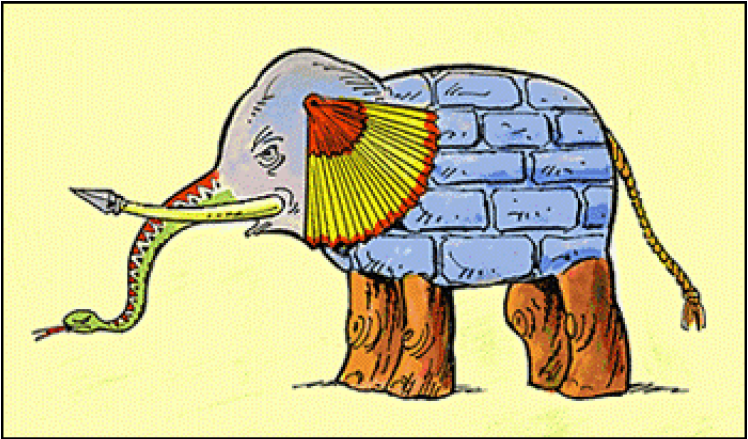
\includegraphics[width=.8\textwidth]{figures/Elefante}
        \end{center}
        \caption {El elefante de Saxe}
        \label{elefante-saxe}
    \end{figure}

    Se usa la analogía para ejemplificar el hecho de que haya varias definiciones diferentes de lo que es SOA en si, porque se le ha definido como patrón de diseño o como una filosifía de desarrollo, siendo esta última la definición adoptada para el trabajo descrito en el presente informe.
    
    También se puede usar dicha analogía para ejemplificar cómo las (potenciamente) distintas vistas pueden interactuar con el controlador y este a su vez con el modelo.


    \section{Autenticación Basada en \textit{Tokens}}
    
    Es una forma de autenticación ligera, que va de la mano con SOA, que usa \textit{tokens}, o fichas, cifradas para la verificación de usuarios. Estas fichas son almacenadas en el cliente y enviadas en cada una de los \textit{requests} que realiza el navegador, la ficha es decifrada y se verifican las credenciales del usuario en cuestión\cite{TOKEN-tokenbasedauth}.
    
    \begin{figure}
        \begin{center}
            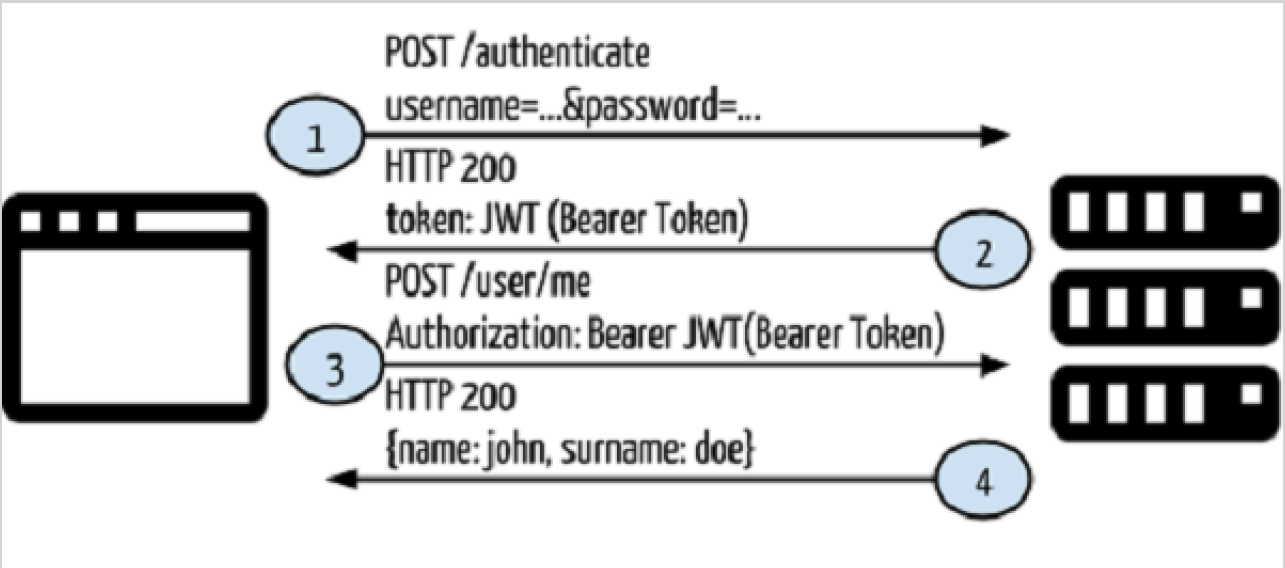
\includegraphics[width=.8\textwidth]{figures/tokenbarequest}
        \end{center}
        \caption{Autenticacion basada en fichas.}
    \end{figure}
    
    Entre los datos almacenados en las fichas pueden estar:
    
    \begin{itemize}
        \item Nombre de usuario.
        \item Fecha de autenticación.
        \item Fecha de caducidad de la ficha.
    \end{itemize}
    
    Estas son cifradas en el servidor bajo una clave secreta elegida por el mismo servidor y que se usa para el posterior decifrado de las fichas.
    
    Todo esto permite que el servidor no se sobrecargue con variables de estado o de sesión por cada usuario autenticado en un momento dado y además permite la portabilidad desesada para el sistema, como muestra en la figura.
    
    \begin{figure}
        \begin{center}
            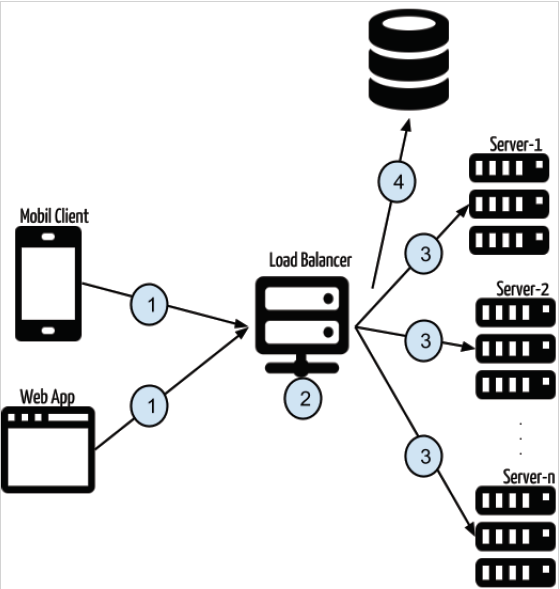
\includegraphics[width=.8\textwidth]{figures/tokenbaservers}
        \end{center}
        \caption{Portabilidad de la Autenticación Basada en Fichas.}
    \end{figure}
    
\pagebreak